%%%%%%%%%%%%%%%%%%%%%%%%%%%%%%%%%%%%%%%%%
% Short Sectioned Assignment
% LaTeX Template
% Version 1.0 (5/5/12)
%
% This template has been downloaded from:
% http://www.LaTeXTemplates.com
%
% Original author:
% Frits Wenneker (http://www.howtotex.com)
%
% License:
% CC BY-NC-SA 3.0 (http://creativecommons.org/licenses/by-nc-sa/3.0/)
%
%%%%%%%%%%%%%%%%%%%%%%%%%%%%%%%%%%%%%%%%%

%----------------------------------------------------------------------------------------
%	PACKAGES AND OTHER DOCUMENT CONFIGURATIONS
%----------------------------------------------------------------------------------------

\documentclass[paper=a4, fontsize=12pt]{scrartcl} % A4 paper and 11pt font size

\usepackage[T1]{fontenc} % Use 8-bit encoding that has 256 glyphs
\usepackage{fourier} % Use the Adobe Utopia font for the document - comment this line to return to the LaTeX default
\usepackage[english]{babel} % English language/hyphenation
\usepackage{amsmath,amsfonts,amsthm} % Math packages

\usepackage{sectsty} % Allows customizing section commands
\allsectionsfont{\centering \normalfont\scshape} % Make all sections centered, the default font and small caps

\usepackage{graphicx}

\usepackage[a4paper,lmargin=2.5 cm,rmargin=2 cm,tmargin=2 cm,bmargin=2 cm]{geometry}

\usepackage{fancyhdr} % Custom headers and footers
\pagestyle{fancyplain} % Makes all pages in the document conform to the custom headers and footers
\fancyhead{} % No page header - if you want one, create it in the same way as the footers below
\fancyfoot[L]{} % Empty left footer
\fancyfoot[C]{} % Empty center footer
\fancyfoot[C]{\thepage} % Page numbering for right footer
\renewcommand{\headrulewidth}{0pt} % Remove header underlines
\renewcommand{\footrulewidth}{0pt} % Remove footer underlines
\setlength{\headheight}{13.6pt} % Customize the height of the header

\usepackage{chngcntr}
%\numberwithin{equation}{section} % Number equations within sections (i.e. 1.1, 1.2, 2.1, 2.2 instead of 1, 2, 3, 4)
%\numberwithin{figure}{section} % Number figures within sections (i.e. 1.1, 1.2, 2.1, 2.2 instead of 1, 2, 3, 4)
%\counterwithout{figure}{section}
%\numberwithin{table}{section} % Number tables within sections (i.e. 1.1, 1.2, 2.1, 2.2 instead of 1, 2, 3, 4)

\setlength\parindent{0pt} % Removes all indentation from paragraphs - comment this line for an assignment with lots of text

\usepackage{amsmath}
\usepackage{float} % To firce the location of figure
\usepackage{subfigure} %For side-by-side figures
\usepackage{lettrine}
%\usepackage{lipsum}
\usepackage{epstopdf} %To read *.eps Files
\usepackage{listings} % To include source codes in LATEX document
\usepackage{mathrsfs} % To include script fonts. use \mathscr{}
\usepackage{courier} % To write in courier fornt
\usepackage{mathtools} % For mat symbols
\usepackage{xfrac} % For \sfrac{}{}
%----------------------------------------------------------------------------------------
%	TITLE SECTION
%----------------------------------------------------------------------------------------

\newcommand{\horrule}[1]{\rule{\linewidth}{#1}} % Create horizontal rule command with 1 argument of height

\title{	
\normalfont \normalsize 
\textsc{Wright State University\\ Department of Mechanical and Materials Engineering} \\ [25pt] % Your university, school and/or department name(s)
\horrule{0.5pt} \\[0.4cm] % Thin top horizontal rule
\huge ME7060 - Structural Reliability \\ % The assignment title
\LARGE Project Proposal
\horrule{2pt} \\[0.5cm] % Thick bottom horizontal rule
}

\author{Koorosh Gobal} % Your name

\date{\normalsize\today} % Today's date or a custom date

\begin{document}

\maketitle % Print the title

%----------------------------------------------------------------------------------------
%	PROBLEM 1
%----------------------------------------------------------------------------------------
\section*{Fluid-Structure Interaction Based Reliability Analysis}
The wings are one of the important parts of a fixed-wing aircraft. When the aircraft travels forwards, air flows over the wings which have airfoil shape to create lift. Whether flexible or rigid, most wings, have a frame to give them their shape and to transfer lift from the wing surface to the fuselage. The basic structural elements are one or more spars running from root to tip, and many ribs running from the leading (front) to the trailing (rear) edge as shown in Figure ~\ref{fig:wing_box}.
%
\begin{figure}[H]
	\centering
    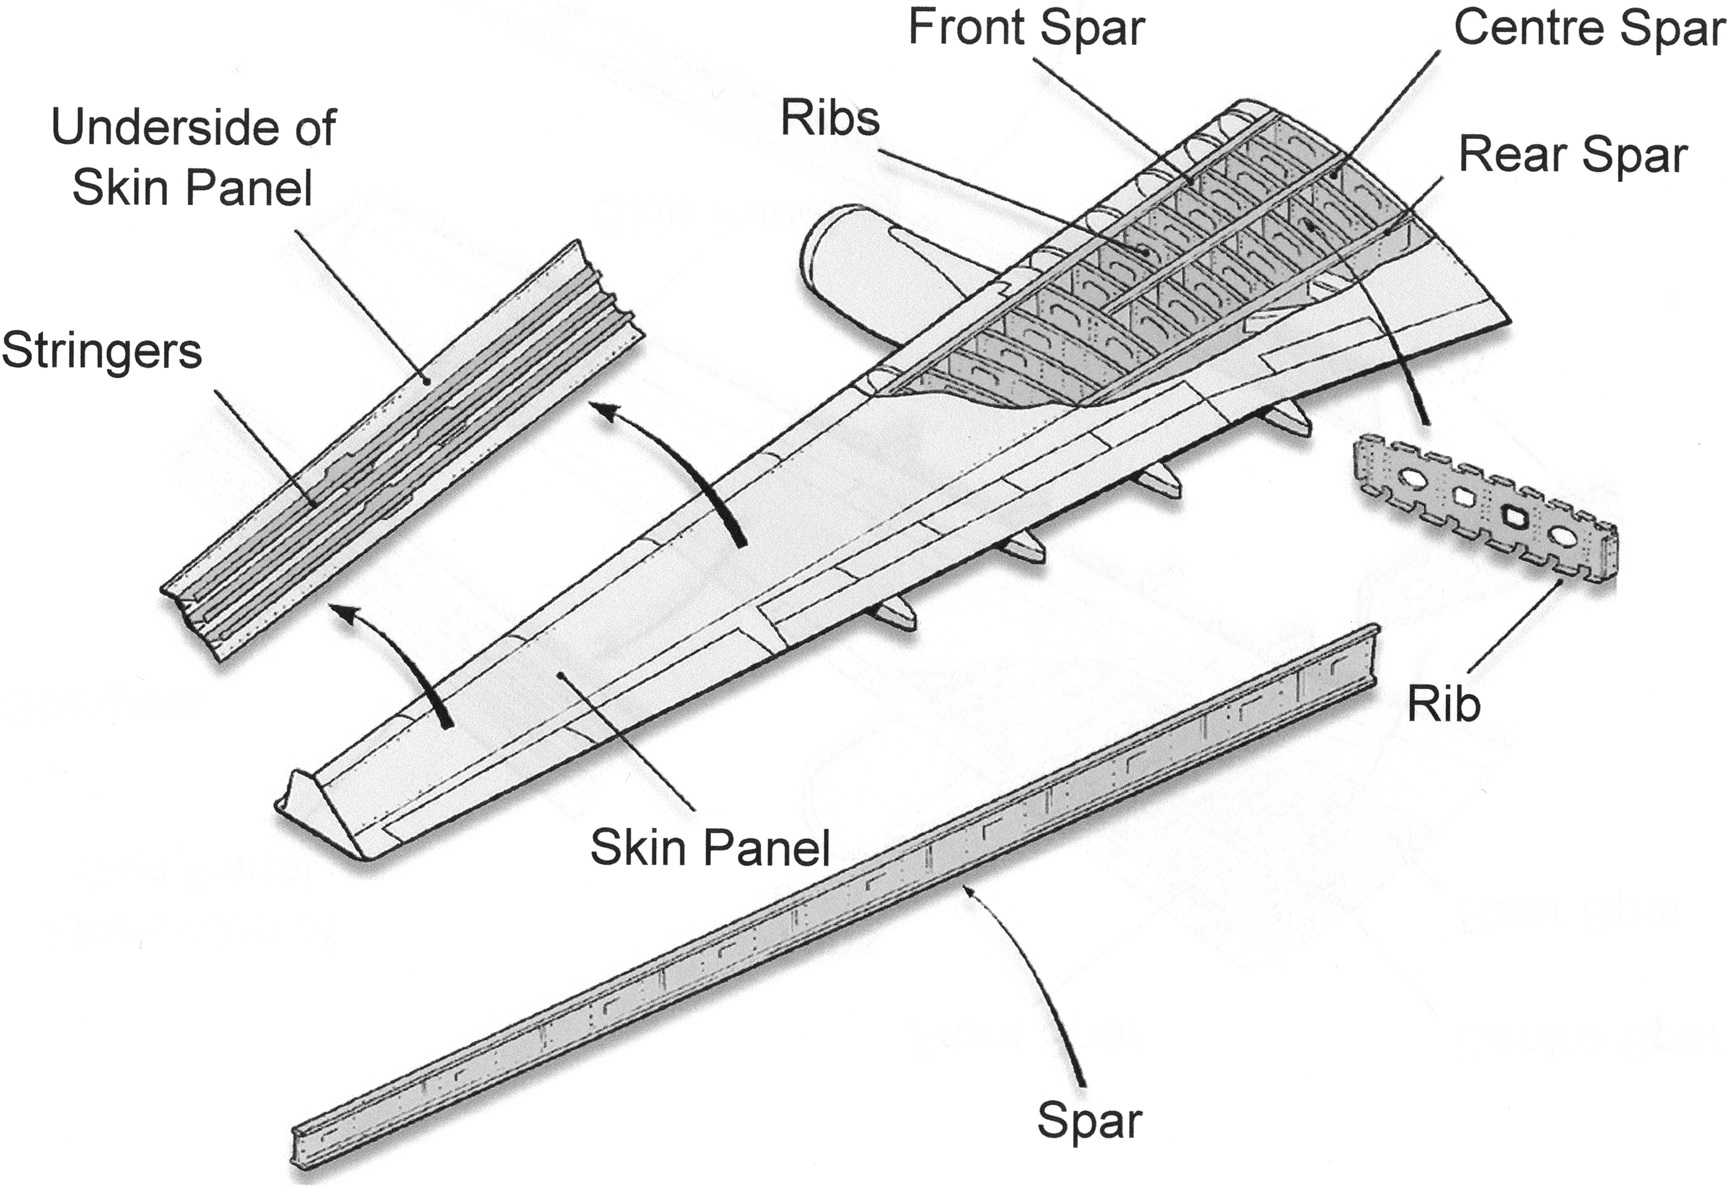
\includegraphics[width=10cm]{wing_box.jpg}
    \caption{Wing-box structure.}
    \label{fig:wing_box}
\end{figure}
%
Wings deform due to the aerodynamic forces which causes the change in the angle of attack and hence change the aerodynamic loading. Wing structure can be modeled using different fidelities. The highest fidelity models are generated using composite and brick elements. The next stage is using spars and ribs followed by modeling the entire wing as a single cantilever beam. In this research we chose the lowest fidelity model (cantilever beam) to represent the wing structure. Therefore, we can investigate different methods of reliability analysis instead of spending time on finite element simulation. The methods can be extended to a wing-box structure modeled with spars and ribs (ICW model). In this research, we will use \emph{Nastran} finite element package to get the structural response. The structure is modeled using \texttt{CBAR} elements. It should me pointed out that the flow and structure are modeled in 2D domain.
%
\begin{figure}[H]
	\centering
    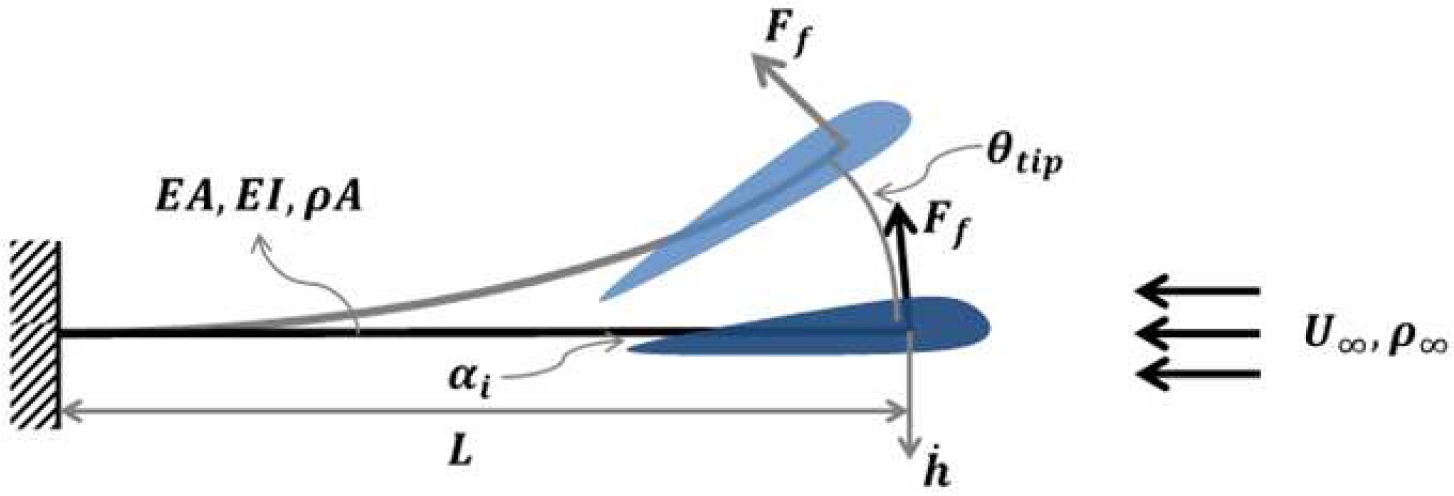
\includegraphics[width=10cm]{problem_discription.jpg}
    \caption{Simplified wing model.}
    \label{fig:problem_discription}
\end{figure}
%
The loading on the structure comes from the aerodynamic forces acting on the airfoil mounted at the end of the beam. The lift force can be calculated by solving the flow field over the airfoil and calculating the pressure profile. These will provide the force and moment applied on the wing structure. These forces can be used to calculate the stress in the wing which is chosen as our limit-state function for the reliability analysis as shown in Equation \eqref{eq:limit_state}.
%
\begin{gather}
	g\left( \bar{X} \right) = 
	\sigma\left( E,I,L,\alpha_\infty,U_\infty,\bar{u}_\infty,\rho_\infty \right)
	- \sigma_{allowable}
	\label{eq:limit_state}
\end{gather}
%
As shown in Equation \eqref{eq:limit_state}, the stress in wing depends on seven variables as specified below
%
\begin{enumerate}
	\item E \quad : \quad Modulus of elasticity of wing structure
	\item I \quad : \quad Area moment of inertia of wing structure
	\item L \quad : \quad Length of wing
	\item $\alpha_\infty$ \quad : \quad Angle of flow coming to the wing
	\item $U_\infty$ \quad : \quad Velocity of flow coming to the wing
	\item $\bar{u}_\infty$ \quad : \quad Sudden fluctuation in speed
	\item $\rho_\infty$ \quad : \quad density of fluid around the wing
\end{enumerate}
%
There are different theories that can be used to calculate the aerodynamic response of the system. \emph{Potential flow} describes the velocity field as the gradient of a scalar function: the velocity potential. As a result, a potential flow is characterized by an irrotational velocity field, which is a valid approximation for several applications such as aerofoils, water waves, electroosmotic flow, and groundwater flow. Nastran has the capability of using potential flow theory, \emph{panel method}, to solve the current aeroelastic problem. Therefore, the $\beta$ value can be calculated using reliability algorithms by calling Nastran to calculate the values for limit-state function and its gradients.\\

Another approach is to use \emph{Euler equations} to solve the flow field. Euler equations are a set of equations governing inviscid flow. The equations represent conservation of mass (continuity), momentum, and energy, corresponding to the Navier-Stokes equations with zero viscosity and heat conduction terms.
%
\begin{subequations}
\begin{gather}
	\dfrac{\partial \rho}{\partial t} + 
		\sum_{i=3}^3 \frac{\partial \left( \rho u_i \right)}{\partial x_i} = 0
	\\
	\dfrac{\partial \left( \rho u_j \right)}{\partial t} + 
		\sum_{i=3}^3 \frac{\partial \left( \rho u_i u_j \right)}{\partial x_i} + 
		\dfrac{\partial p}{\partial x_j} = 0
\end{gather}
\end{subequations}
%
Euler equations is a special/limiting case of the more general {non-linear} Navier-Stokes equation. Therefore, using it will give us more insight about the problem compared to potential flow. To solve the Euler equations around the airfoil a separate CFD solver is needed to calculate the pressure profile around the airfoil. In this research we are planing to connect an open source CFD solver (OpenFOAM) to solve the flow.
% ---------------------------------------------------------------------------- %
\end{document}